%\chapter{Problem\'atica de la Individualizaci\'on de Filamentos a partir de un Grafo}
\chapter{Antecedentes}
\label{chap:cap2}

%problema previo, o problema 0 que consiste en la generaci\'on de un grafo a partir de una imagen que contenga una red, que en este caso, representaria a una red de filamentos. 

En base lo expuesto en el cap\'itulo \ref{chap:stateoftheart}, para el enfoque de utilizar grafos para la individualizaci\'on de filamentos existe una brecha entre la obtenci\'on del grafo y su an\'alisis. Este paso previo, la extracci\'on de un grafo a partir de una imagen, lo denominamos como el problema previo o problema 0 y consiste en extraer un grafo $G = (V,E)$ de una imagen tal que $G$ sea un grafo simple, no dirigido, ponderado, conectado o desconectado, con o sin ciclos. Esto implica que exista a lo m\'as 1 arista por cada par de nodos adyacentes, prohibi\'endose la existencia de nodos conectados consigo mismos. Se definen los v\'ertices/nodos del grafo $G$ como $V(G)$ y las aristas de $G$ como $E(G)$. 
Que el grafo $G$ sea ponderado se puede definir en $\forall e \in \quad E(G) \quad  \exists $ caracter\'isticas asociadas que se expresan como caracter\'isticas geom\'etricas, topol\'ogicas, espaciales y/u otras. Es importante evitar que $G$ sea un grafo completo, dado que con n nodos/v\'ertices $G$ tenga $\frac{n(n-1)}{2}$ aristas. 

Algunas de las dificultades involucradas en la extracci\'on de informaci\'on a partir de una imagen se encuentran en los m\'etodos presentados en el cap\'itulo \ref{chap:stateoftheart}, dentro de las que destacan el ruido y la resoluci\'on. Un ejemplo de aquello se observa en la figura \ref{fig:NoConsenso}.

\begin{figure*}[h]
    \begin{tabular}{c c c}
        \multirow[c]{2}{*}[2.5cm]{
        \begin{subfigure}[t]{0.4\textwidth}
        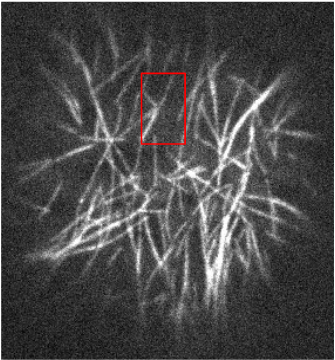
\includegraphics[scale=0.5]{imagenes/NoConsenso.png}
        \caption{Microt\'ubulos en planta {\it Marchantia}.\\Fuente: Paula Llanos}
        \label{fig:NoConsensoGeneral}
        \end{subfigure}  
        }
        &
        \multirow[c]{2}{*}[2cm]{
        \begin{subfigure}[t]{0.25\textwidth}
        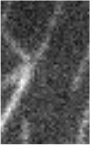
\includegraphics[]{imagenes/NoConsenso2.png}
        \caption{Secci\'on resaltada en rojo de \ref{fig:NoConsensoGeneral}}
        \label{fig:NoConsensoRect}
        \end{subfigure}
        }
        &
        \begin{subfigure}[t]{0.21\textwidth}
        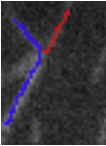
\includegraphics[scale=0.8]{imagenes/NoConsenso3.png}
        \caption{Opci\'on 1 de microt\'ubulos en \ref{fig:NoConsensoRect}}
        \label{fig:NoConsensoOpcion1}
        \end{subfigure} \\
        & &
        \begin{subfigure}[b]{0.21\textwidth}
        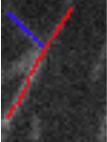
\includegraphics[scale=0.8]{imagenes/NoConsenso4.png}
        \caption{Opci\'on 2 de microt\'ubulos en \ref{fig:NoConsensoRect}}
        \label{fig:NoConsensoOpcion2}
        \end{subfigure} \\
    \end{tabular}
    
    \caption{Dificultad de individualizaci\'on que enfretan los expertos al analizar manualmente una imagen de filamentos, en particular, microt\'ubulos.}
    \label{fig:NoConsenso}
\end{figure*}

Mientras que el ruido ha sido estudiado en la literatura, el problema de resoluci\'on de filamentos depende principalmente de la capacidad del microscopio que se utilice. Como se menciona en la introducci\'on, el l\'imite m\'aximo de resoluci\'on, denominado $\frac{\lambda}{2}$ determina  el tama\~no m\'inimo que 2 objetos que se encuentren juntos pueden tener para no observarse como un \'unico elemento. Lo anterior sucede para algunos tipos de filamentos como los microt\'ubulos que pueden medir tan solo 25 nan\'ometros, lo que se encuentra por debajo de $\frac{\lambda}{2}$ para diversos microscopios. 



Una vez obtenido el grafo que representa una red de filamentos, el problema siguiente se encuentra en el que 2 expertos pueden discernir con respecto a los filamentos identificables en una imagen, por lo que no es posible conocer a priori del origen y el final de un filamento, para las resoluciones actuales de las imagenes obtenidas a partir de la microscop\'ia. Se añade como dificultad que dada la representaci\'on de un filamento en un grafo se basa en un conjuntos de aristas adyacentes (denominadas caminos), pudiendo significar la b\'usqueda en un universo de hasta $n!$ posibles combinaciones.

A partir del problema anterior, el problema final lo constituye la elecci\'on del subconjunto de caminos, que debe ser seleccionado entre el total de caminos que representan soluciones factibles. Esto implica que el problema no solo sea un problema combinatorial de generar soluciones factibles a partir del conjunto de aristas, sino que adem\'as debe considerar la discriminaci\'on entre estos para obtener el subconjunto de mayor calidad, pudiendo representarse como un problema de optimizaci\'on combinatorial.

Los 3 problemas presentados se formalizan a continuaci\'on.

%problema previo
%presentar el problema previo, como un puente necesario en la automatizaci\'on de la extracci\'on,  para analizar un grafo que representa la red de filamentos, que de lo contrario tendria que ser realizado a mano, implicando que la persona realizando el análisis podría llevar a cabo la individualizaci\'on de filamentos en el mismo acto.

\section{Generaci\'on de un Grafo desde una Imagen}
La extraci\'on o generaci\'on de un grafo que representa una red de filamentos a partir de una imagen es el paso que define la cantidad de informaci\'on disponible para llevar a cabo la individualizaci\'on de filamentos. La importancia de este procedimiento radica en que a partir de la imagen es posible obtener una cantidad de caracter\'isticas de distinta \'indole, lo que permite en etapas posteriores desagregar el grafo $G$ en subgrafos mediante la clasificaci\'on de nodos y/o aristas, efectivamente disminuyendo el espacio de b\'usqueda. Con las herramientas actuales disponibles en la literatura es posible realizar la extracci\'on de una red de filamentos con algún nivel de informaci\'on como en \cite{xu2015soax}. Sin embargo, las transformaci\'on de aquella red a un grafo, as\'i como la incorporaci\'on de las caracter\'isticas y/o propiedades hacia el grafo son un procedimiento no automatizado, por lo que el esfuerzo que el experto debe realizar es cercano a individualizar los filamentos de manera manual.

Es posible distinguir en 2 conjuntos los m\'etodos utilizados para extraer la informaci\'on escencial que permite la construcci\'on de un grafo a partir de una imagen, como lo son los nodos y las aristas. Estos conjuntos son los que se basan en esqueletonizaci\'on\cite{lavado2018comparacion} y los que no. 

%En este trabajo se presenta un enfoque del segundo tipo.


\subsection{Extracci\'on de un Grafo mediante Esqueletonizaci\'on}


\subsection{Generador Aproximado de Grafos a partir de una Imagen}

Con el fin de aportar en automatizar la extracci\'on de informaci\'on de una imagen para la generaci\'on de un grafo que representa una red de filamentos, se construye una herramienta que en base a una imagen, construye lo que se denomina un grafo aproximado de la red de filamentos. El procedimiento consta de 3 pasos:
% explicar que el hecho de G completo mediante lo q la arista es al problema de identificación de filamentos
%presento el extractor aproximado de grafos, la noción de puntos cluster/superPixels/blobs y el centro de masa como representante, dado que se puede obtener de forma simple mediante los "image moments". Además, distintos niveles de image moments permiten obtener información adicional útil en la descripción del cluster.

\begin{enumerate}
    \item Se generan clusters, tambi\'en llamados {\it Super Pixels} mediante una agrupaci\'on en base a un kernel 3x3, que busca separar de forma local los pixels que corresponden a {\it background} respecto a los de {\it foreground}, siendo estos \'ultimos los que concentran el inter\'es para an\'alisis. La creaci\'on de clusters permite establecer la primera informaci\'on de vecindarios.
    \item Cada cluster es representado por un nodo, ubicado en el centro de masa del {\it super pixel}. En conjunto con el centro de masa es posible obtener informaci\'on geom\'etrica mediante los {\it raw image moments}\cite{chaumette2004image} del cluster. En este punto tambi\'en se procede a realizar una uni\'on de clusters que evita la creaci\'on de aristas demasiado cortas entre 2 nodos, as\'i como la identificaci\'on de ciclos triangulares, que generan aberraciones en el grafo generado.
    \item A partir de la informaci\'on de vecindario de los nodos definitivos obtenidos en el paso anterior, se generan aristas entre nodos vecinos. Se obtiene el largo e  informaci\'on angular para cada arista creada. %Esta \'ultima es utilizada m\'as adelante para definir puntos de partida de las hormigas.
\end{enumerate}

Se define como generador {\it aproximado} de grafos debido a que puede sufrir de peque\~nas desviaciones en la ubicaci\'on de los nodos y las aristas con respecto a lo que otras herramientas de esqueletonizaci\'on e identificaci\'on de intersecciones en conjunto pueden hacer en la misma tarea. Uno de los objetivos en la creaci\'on del generador {\it aproximado} de grafos se debe a que facilita el uso de im\'agenes encontradas en el estado del arte.

%La noción ppal es generar vecindarios, ya que el grafo debe contener información topológica como geométrica, ya que cada será la base para distintos criterios de categorización durante el proceso de individualización de filamentos. 
El objetivo principal del generador en s\'i es el crear vecindarios, siendo esto la base de la informaci\'on topol\'ogica, que se suma a la informaci\'on geom\'etrica que se construye en los pasos descritos anteriormente. Un ejemplo de esto pueden ser los ciclos, dado que el n\'umero de vecinos que constituye el grado de cada nodo permite identificar la existencia de ciclos\cite{wilson1979introduction}, que son discriminantes importantes dependiendo del filamento que se analice. 

%se destaca dentro de los criterios del generador aproximado de grafos a partir de una imagen se busca evitar perder información de la imagen, así como tener un costo computacional bajo, en conjunto con disminuir la interacción del usuario. 

Otros objetivos del generador aproximado de grafos son evitar la perdida de informaci\'on durante la obtenci\'on del grafo, y evitar la perdida de informaci\'on. Esto \'ultimo puede suceder si se utiliza esqueletonizaci\'on de la imagen para obtener el grafo, dado que mediante el adelgazamiento utilizado se rompe la relaci\'on entre los p\'ixeles que conforman el elemento que se adelgaza y los p\'ixeles que constituyen el esqueleto obtenido. Se analizaron diversos filtros para obtener informaci\'on dentro de los que destacan {\it Gabor Gaussian kernels}, siendo descartado ya que se pierden detalles mediante el uso de {\it blurring} \cite{kerkeni2016coronary}, mientras que el filtro {\it Anistropic Diffusion} fue descartado por requerir de múltiples parámetros. En la misma linea, la elecci\'on de {\it image moments}\cite{flusser2009moments} se fundamenta en el estudio del filtro Frangi para {\it Veselness}\cite{frangi1998multiscale}\cite{fu2018frangi}, utilizado para filtrar estructuras alargadas, como lo son arterias y venas. Este filtro se basa en los eigenvectores y eigenvalores de la matriz Hessiana (ecuaci\'on \eqref{eq:HessianMat}) obtenida despu\'es de filtrar una imagen, obteniendo el {\it veselness value} o valor de cuan alargada es una estructura. 

\begin{equation}
    \label{eq:HessianMat}
    H = \begin{bmatrix}
        H_{xx} & H_{xy} \\
        H_{xy} & H_{yy} 
        \end{bmatrix}
\end{equation}

Un respuesta de {\it veselness value} que denota una estructura alargada se obtiene si los 2 eigenvalores, $\lambda_1$ y $\lambda_2$ ($|\lambda_2| \geq |\lambda_1|$) satisfacen $|\lambda_1| \approx 0 $ y $|\lambda_2| \gg |\lambda_1|$. Los eigenvalores se obtienen mediante la ecuaci\'on \ref{eq:lambdaFrangi}.

\begin{equation}
    \label{eq:lambdaFrangi}
    \lambda_{1,2} = \dfrac{(H_{xx} + H_{yy}) \pm \sqrt{(H_{xx} - H_{yy})^{2} + 4\cdot H_{xy}^{2}     } }{2}
\end{equation}

Otra forma de obtener los valores de lambda de la ecuaci\'on \ref{eq:lambdaFrangi} es utilizando los {\it central image moments} o momentos centrales, que derivan de los {\it raw image moments} obtenidos en el segundo paso del generador aproximado de grafos. Se define un {\it raw image moment} de orden $p+q$ para una imagen en la ecuaci\'on \eqref{eq:rawImageMoment}, donde $f(x,y)$ corresponde a la intensidad de la imagen en un punto (x,y). El {\it raw moment} $M_{00}$ refleja la "masa" de la imagen, correspondiendo al \'area o volumen si se trata de una imagen binaria. 

Para el c\'alculo de los momentos centrales se agregan los componentes del centroide, $\overline{x}$ e $\overline{y}$, basados en los {\it raw moments}, como indican las ecuaciones \eqref{eq:avgFromRawMomts} y \eqref{eq:centralImageMoment}.

\begin{subequations}
\begin{equation}
    \label{eq:rawImageMoment}
    M_{pq} = \sum\limits_{x} \sum\limits_{y} x^p \cdot y^q \cdot f(x,y)
\end{equation}
\begin{equation}
    \label{eq:avgFromRawMomts}
    \overline{x} = \frac{M_{10}}{M_{00}}, \quad
    \overline{y} = \frac{M_{01}}{M_{00}}
\end{equation}
\begin{equation}
    \label{eq:centralImageMoment}
    \mu_{pq} = \sum\limits_{x} \sum\limits_{y} (x - \overline{x})^{p} \cdot (y - \overline{y})^{q} \cdot f(x,y)
\end{equation}
\end{subequations}

As\'i, es posible construir una matriz de covarianza, equivalente a la matriz hessiana en la ecuaci\'on \eqref{eq:HessianMat}, utilizando los momentos centrales de segundo orden, $\mu_{20}$, $\mu_{02}$ y $\mu_{11}$ divididos por el momento central de orden cero $\mu_{00}$ (ecuaciones \eqref{eq:mu20}, \eqref{eq:mu02} y \eqref{eq:mu11}), obteniendo los eigenvalores mediante la ecuaci\'on \eqref{eq:lambdaMoments}.

\begin{subequations}
\begin{align}
    \mu_{20}^{\prime} &= \frac{\mu_{20}}{\mu_{00}} = \frac{M_{20}}{M_{00}} - \overline{x}^{2} \label{eq:mu20} \\
    \mu_{02}^{\prime} &= \frac{\mu_{02}}{\mu_{00}} = \frac{M_{02}}{M_{00}} - \overline{y}^{2} \label{eq:mu02} \\
    \mu_{11}^{\prime} &= \frac{\mu_{11}}{\mu_{00}} = \frac{M_{11}}{M_{00}} - \overline{x}\cdot\overline{y} \label{eq:mu11}
\end{align}

\begin{equation}
    \label{eq:covMatLambda}
    cov[f(x,y)] = \begin{bmatrix}
        \mu_{20}^{\prime} & \mu_{11}^{\prime} \\
        \mu_{11}^{\prime} & \mu_{02}^{\prime} 
        \end{bmatrix}
\end{equation}

\begin{equation}
    \label{eq:lambdaMoments}
    \lambda_{1,2} = \dfrac{(\mu_{20}^{\prime} + \mu_{02}^{\prime}) \pm \sqrt{(\mu_{20}^{\prime} - \mu_{02}^{\prime})^{2} + 4\cdot \mu\prime_{11}^{2} }}{2}
\end{equation}
\end{subequations}

La recopilaci\'on de informaci\'on de esta forma permite su posible uso en las etapas de la individualizaci\'on de filamentos.


\subsubsection{Heurística para limitar el n\'umero de nodos}
%numero de nodos depende de apMaxThickness, q representa la resoluci\'on, es decir, cuantos micrometros se observan por pixel.
En concordancia con lo expresado al inicio de este cap\'itulo, es necesario evitar que el grafo $G$ extra\'ido a partir de la imagen, sea completo. Con el fin de evitar esa condici\'on se desarrollan las estrategias mencionadas en el segundo paso del generador aproximado de grafos. Para la construcci\'on del grafo aproximado, el usuario dispone de un par\'ametro denominado {\it maxThickness} asociado al grosor m\'aximo que un filamento en la imagen de entrada puede tener. Se define que la distancia m\'inima entre 2 nodos no podr\'a ser inferior a un porcentaje de {\it maxThickness}, variando el porcentaje depenendiendo de lo que el usuario indique que se esta observando (microt\'ubulo, neurona, ret\'iculo u otro). En caso de no superar el umbral, los nodos se unen. Otra componente de la heur\'istica que limita la cantidad de v\'ertices es el n\'umero m\'inimo de p\'ixeles que cada cluster debe contener, la cual debe ser mayor que 1.5 veces {\it maxThickness}. Esto con la finalidad de evitar clusters muy peque\~nos, que lleva a la creaci\'on de demasiados nodos. 

%Finalmente, se hace un an\'alisis topol\'ogico que evita la formaci\'on de ciclos triangulares
 

%A su vez, otro motivo para evitar que $G$ sea un grafo completo radica en que para los filamentos observados en la naturaleza no es una condici\'on comun... no encuentro la fuente de esto

%Un grafo completamente conectado puede tener n(n-1)/2 aristas, lo que para un n muy grande puede implicar un costo computacional se aplicó como estrategía: Node Pruning: parametro apMaxThickness y connectivityThreshold manuales. Arbitrariamente n\textdegree neighbors > 2. también se fija un límite de memoria ram


% ambas opciones generan degeneraciones/deformaciones q afectan
\section{Exploraci\'on del Espacio de Soluciones}
definir que los segmentos/caminos/path son conjuntos de aristas adyacentes conectadas, o de nodos ..., que cumplen con restricciones, como la restricción angular o restricciones de ciclos (formula matem\'atica) y que los filamento son elegidos entre los caminos de mayor calidad
Un camino simple es equivalente a un \'arbol simple, ac\'clico...


En un grafo con n aristas, en el cual se desconoce el origen y el final los caminos, el n\'umero de combinaciones crece exponencialmente (agregar \cite{buchin2007number}\cite{biswas2012hamiltonian}). Denominamos todas estas opciones de caminos como el conjunto $P$, del cual debemos extraer un subconjunto $P'$ mediante una estrategia que permita realizar esto en tiempo polinomial independientemente de la cantidad de aristas del grafo.

\begin{equation}
p = (e_1, e_2,..., e_n)\\
p = ((v_1,v_2), (v_2,v_4),..., (v_n-1,v_n))
\label{eq:path}
\end{equation}

% explicar define
El m\'etodo presentado en \cite{breuer2015define} se basa en lo definido por \cite{lin2006vertex}, indicando que dado un problema de {\it covering}, existe un {\it set system}$(S,C)$, donde S es el conjunto total y finito de sets, y C es un conjunto de subsets pertenecientes a S. En el caso espec\'ifico del {\it Minimum Set Cover}(SC), el objetivo es encontrar un subconjunto $C'$ de $C$ tal que cada elemento de $S$ pertenezca al menos 1 vez a uno de los miembros de $C'$.

Para un {\it set system}$(S,C)$ que pueda ser representando por un \'arbol $T$, es posible modificar la definici\'on de $S$ al conjunto de nodos que componen un grafo $G$ y que cada subset $c \in C$ representa un camino\eqref{eq:path} simple en $G$. Se destaca que no necesariamente estar\'an todos los caminos simples de $G$ est\'an representados en $C$. Esta representaci\'on de {\it covering} de caminos, o {\it Path Cover}, es denominada {\it Vertex Covering by Paths on Graphs}(VcpG) y difiere de un {\it Path Cover} tradicional al permitir caminos que compartan nodos. Luego, para el caso de \'arboles, VcpG se renombra a VcpT ({\it Vertex Covering by Paths on Trees}), y si se reemplazan los nodos por aristas, lo no genera cambios significativos en el planteamiento del problema, se denomina EcpT {\it Edge Covering by Paths on Trees}. %recordar mas adelante como posible perdida de soluciones factibles


Lo anterior establece las bases para que los autores de DeFiNe\cite{breuer2015define} utilicen EcpT como base, teniendo un m\'aximo de caminos $n(n)-1/2 = \mathcal{O}(n^{2})$, con una complejidad $\mathcal{O}(n^{4})$ para obtener esos caminos, para caminos que no comparten nodos o aristas, es decir, no se sobrelapan.

La obtenci\'on de caminos a partir de un \'arbol $T$ que representa un grafo $G$ se realiza mediante la divisi\'on continua del \'arbol en m\'ultiples bosques, hasta que los bosques resultantes sean s\'olo caminos simples.

%aca entran las formas de obtener esos arboles simples y bosques, con las heuristicas de define
...


% Comparándose con define,
el problema acá está en la generación de P' subconjunto de P (caminos totales) , ya que al usar una sola propiedad, como lo puede ser el ángulo entre aristas, el largo o el ancho, se pierden soluciones. Ejemplo camino verde en Spinning Marchantia (imagenes)

% Heurística: hay alguna aca? pareciera solo satisfacci\'on de restricciones
% garantizar que al satisfacer las restricciones los caminos son solo soluciones factibles y que la unión de caminos también entrega múltiples opciones de filamentos, los que deben ser medidos para determinar cual es mejor




\section{Modelo de Optimización}
%dado que se tienen muchos filamentos, se debe evaluar cual es mejor. Explicar como propiedades topológicas y geométricas tienen. Y como se ponderan para un peso que será minimizado o maximizado

En base a lo recopilado en las secciones previas de esta investigaci\'on, es posible destacar los siguientes aspectos al problema a resolver:

\begin{itemize}
    \item Se desconoce a priori el n\'umero de filamentos a buscar, dado que una imagen puede tener individualizaciones distintas para 2 expertos.
    \item Generalmente, se busca individualizar m\'as de un filamento por imagen, lo que conlleva a elegir los mejores filamentos entre las soluciones que se encuentren.
    \item El uso de un grafo para representar la red de filamentos puede implicar que las combinaciones de soluciones crezcan de manera exponencial.
\end{itemize}

Lo anterior implica que el problema de identificar filamentos a partir de un grafo puede ser clasificado como un problema de optimizaci\'on de restricciones\cite{blum2011hybrid}.

Un problema de optimización de restricciones, (COP por su sigla en ingl\'es) puede ser representado como $P = (S, \Omega, F)$, donde S es el espacio de soluciones, definido por un conjunto discreto de variables $X = 1 \dotsc n$, con valores $v_{i}^{j} \in D_{i} = \{v_{i}^{1} \dotsc  v_{i}^{|D_{i}|}\}$. Se define como una variable {\it instanciada} la asignaci\'on a $X_i$ de un valor $v_{i}^{j} \in D_i$. Una solución candidata $s \in S$ es una soluci\'on factible si satisface las restricciones del set $\Omega$. La funci\'on objetivo $F: S\rightarrow \mathbb R_{0}^{+}$, es la funci\'on de evaluaci\'on que asigna valores a las soluciones candidatas. Al mismo tiempo, se define $s^{*}$ como una soluci\'on \'optima y $S^{*}$ como un conjunto de soluciones \'optimas, relacionados mediante $s^{*} \in S^{*} \subseteq S $\cite{socha2008ant}.
Esta definici\'on permite aplicar la metaheur\'istica de optimizaci\'on basada en colonia de hormigas (ACO por su sigla en ingl\'es) a un modelo de un {\it COP}.
%COP es un CSP con función objetivo: https://en.wikipedia.org/wiki/Constrained_optimization#Constraint_optimization_problems

\subsection{Metaheur\'istica ACO}
El proposito de la metaheur\'istica ACO es encontrar una soluci\'on o un set de soluciones. Una soluci\'on $s$ consiste en un conjunto de componentes de soluci\'on $c_{ij} \in C, i = 1 \dotsc n, j = 1 \dotsc |D_i|$, por lo que una concatenaci\'on de componentes de soluci\'on forma el camino o {\it tour} que recorre una hormiga, desde un nodo o arista inicial hasta un nodo o arista final. La metaheur\'istica ACO se muestra en el algoritmo \ref{ACO-Algo}. En base a la definici\'on de variable {\it instanciada} del modelo COP, se tiene que la asignaci\'on $X_i = v_{i}^{j}$ es equivalente a seleccionar un componente $c_{ij}$ para una soluci\'on $s$ en ACO.

ACO consiste en un paso de inicializaci\'on y de tres componentes, las que no tienen un orden espec\'ifico: {\it Construccion\_de\_soluci\'on\_de\_cada\_hormiga(),  M\'etodo\_de\_b\'usqueda\_no\_local()} y {\it Actualizaci\'on\_de\_feromonas()}.


\begin{algorithm}[H]
\SetAlgoLined
\KwData{Variables $X_i \dotsc X_n$, dominios $D_1 \dotsc D_n$, Restricciones $\in \Omega$}
\KwResult{conjunto s\textquotesingle $ \subseteq S$ != $\emptyset$, si existen soluciones factibles}
 Ajuste de Par\'ametros \& inicializaci\'on de feromonas \;
 \While{Criterio de finalización no se cumple}{
   Planificaci\'on\_de\_Pasos\;{
   ~ Construccion\_de\_soluci\'on\_de\_cada\_hormiga()\;
   ~ M\'etodo\_de\_b\'usqueda\_no\_local() \% opcional (DaemonActions)\;
   ~ Actualizaci\'on\_de\_feromonas()\;
   }Fin\_Planificaci\'on\_de\_Pasos\;
 }
 \caption{Algoritmo Metaheur\'istica ACO}\label{ACO-Algo}
\end{algorithm}


\subsubsection{M\'etodo Construccion de soluci\'on de cada hormiga}
La elecci\'on de un componente $c_{ij}$ por una hormiga durante la construcci\'on de un camino,
se lleva a cabo mediante el c\'alculo de una probabilidad para cada componente $c_{ij}$ posible de elegir. Este conjunto de vecinos factibles se denomina $N(s^{P}) \subseteq C$. En la probabilidad de selecci\'on influye el camino ya escogido, denominado soluci\'on parcial $s^{P}$. Al comenzar un recorrido, cada hormiga es asignada una arista de acuerdo a la heur\'istica de asignaci\'on, la cual analiza 3 situaciones:
\begin{enumerate}
\item La arista a asignar debe tener al menos uno de sus nodos con grado 1, indicando que es el inicio o final de una parte del grafo.

\item De no haber aristas con esas caracter\'isticas disponibles, se realiza una asignaci\'on inicial de una arista con uno de sus nodos con grado 2 o superior, siempre que uno de los nodos sea la uni\'on de esta arista con otra con la que conformen un \'angulo en el rango $]\theta, MAX\_ANGLE]$. $\theta$ es un umbral que define el \'angulo m\'aximo, en grados, bajo el que se considera que 2 aristas contiguas respetan la rectitud necesaria para formar parte del mismo filamento. $MAX\_ANGLE$ es un umbral que define el \'angulo m\'aximo, en grados, por sobre el cual se descarta de forma absoluta que 2 aristas contiguas forman parte del mismo filamentos. Este rango delimita los pares de aristas que a priori no representan combinaciones que respetan el criterio de rectitud, pero cuya explicaci\'on puede encontrarse en variaciones inducidas durante la extracci\'on del grafo desde la imagen, por lo que es necesario incorporar la exploraci\'on de estos pares de aristas.

\item De no existir aristas con alg\'un nodo que cumpla con los dos criterios previos, es posible asignar una arista aleatoria siempre que esta no forme parte de un camino recorrido por otra hormiga que haya sido evaluado como de buena calidad.
\end{enumerate}

% a diferencia de otros ACO, aca s^P != \emptyset al comienzo
Una vez asignada la primera arista seg\'un la heur\'istica previamente descrita, cada hormiga debe avanzar mediante la elecci\'on de nuevas aristas para a\~nadirlas a su recorrido. Este procedimiento se describe en la ecuaci\'on \eqref{eq:antProbabilities}, que corresponde a la probabilidad de elegir una arista a partir de un conjunto de aristas vecinas (conjunto $N(s^{P})$) dadas la aristas que ya pertenecen a la soluci\'on parcial de la hormiga ($s^P$), mediante la heur\'istica miope (ecuaci\'on \eqref{eq:heuristicaMiope}) que privilegia los candidatos que causen la menor desviaci\'on en la rectitud del camino. Se define que los componentes $c_{ij}$ que aportan con mayor probabilidad a la menor desviaci\'on son aquellos que en conjunto con el \'ultimo elemento elegido por la hormiga en ese punto ($c_{(i-1)j}$) forman un \'angulo en el rango $[0, \theta]$. El criterio de finalizaci\'on para la hormiga corresponde a que el conjunto $N(s^{P}) = \emptyset$.

%P(C_{ij} | s^{P}) = P_{n_{i},n_{j}} = P_{e_{x}}
\begin{equation}
P(c_{ij} | s^{P}) = \frac
        {\tau_{ij}^{\alpha} \cdot \eta_{ij}^{\beta}}
        {\sum\limits_{c_{ij}\in N(s^p)}{\tau_{ij}^{\alpha} \cdot \eta_{ij}^{\beta} } }, \forall c_{ij} \in N(s^{P})
\label{eq:antProbabilities}
\end{equation}

Otro aspecto de la ecuaci\'on \eqref{eq:heuristicaMiope} radica en la posibilidad de elecci\'on de elementos $c_{ij}$ que tienen un \'angulo en el rango $]\theta, \text{MAX\_ANGLE}]$ con el componente de soluci\'on $c_{(i-1)j}$. Esto facilita la exploraci\'on de soluciones/caminos que de forma miope aparecen como de calidad no \'optima, y que para los efectos de este trabajo se denominan como de {\it calidad intermedia}. Esta evaluaci\'on consistente en disminuir la probabilidad de elecci\'on a medida que la diferencia entre el \'angulo que forman $c_{ij}$ y $c_{(i-1)j}$  , y la mitad de $\theta$ se incrementa.


%donde cada uno representa a una arista en esta investigaci\'on, y . Al momento de que la diferencia sea 90\textdegree, la probabilidad de asignaci\'on se reduce al 50\% de la probabilidad de un componente $c_{ij} \in [0, \theta]$.

\begin{equation}
    \eta_{ij} = 
        \begin{cases} 
        \text{MAX\_SCORE si } \measuredangle(c_{ij}, c_{(i-1)j}) \in [0, \theta]\\[3ex]
        
        \text{MAX\_SCORE} \cdot \left(1 - \dfrac{ \left| \measuredangle(c_{ij}, c_{(i-1)j}) - \frac{\theta}{2} \right|} {180} \right)  \text{ si } \measuredangle(c_{ij}, c_{(i-1)j}) \in \quad ]\theta, \text{MAX\_ANGLE}].\\[3ex]
        
        \text{0 en otro caso;}
        \end{cases}
    \label{eq:heuristicaMiope}
\end{equation}

Con la finalidad de cuantificar la calidad de la soluci\'on construida por una hormiga, en cada selecci\'on de arista realizada, se suma el resultado de la heur\'istica miope al valor que la calidad de la hormiga lleva hasta ese punto. Cada hormiga comienza con una calidad 0, que al finalizar el {\it tour} es dividida por el n\'umero de aristas menos 1, para normalizar. Se establece que para ser considerada una soluci\'on de buena calidad, la hormiga debe tener una calidad mayor o igual a $\frac{MAX\_SCORE}{2}$.
    
\subsubsection{M\'etodo de b\'usqueda no local}
Una vez que la hormiga termina un {\it tour}, es posible agregar un m\'etodo de {\it feedback} sobre la calidad del recorrido realizado, basado en l\'ogicas globales/centralizadas que escapan de la b\'usqueda local que realiza cada hormiga. Estos m\'etodos, denominados {\it Daemon Actions} en ingl\'es, permiten en el caso de una metaheur\'istica ACO gen\'erica seleccionar las hormigas de mejor calidad para incrementar las feromonas m\'as alla de lo que la {\it Actualizaci\'on\_de\_feromonas()} lo hace. 

Para la individualizaci\'on de filamentos, la evaluaci\'on global corresponde a eliminar soluciones candidatas que no aporten informaci\'on nueva. A modo de ejemplo, si $s_a$ y $s_b$ son las soluciones de las hormigas $a$ y $b$ respectivamente y cumplen con las siguientes condiciones:

\begin{itemize}
    \item $\forall c_{ij} \in s_a \in [0, \theta]$ y $\forall c_{ij} \in s_b \in [0, \theta]$
    \item $\forall c_{ij} \in s_a$ fueron electos por la hormiga $a$ con $P(c_{ij} | s_{a}^{P}) = 1$ y $\forall c_{ij} \in s_b$ fueron electos por la hormiga $b$ con $P(c_{ij} | s_{b}^{P}) = 1$
    \item $s_a \subseteq s_b$
\end{itemize}

Se tiene que $s_a$ no aporta m\'as informaci\'on que $s_b$, por lo que $s_a$ puede descartarse. Se denomina a $s_b$ como un segmento, el cual se comporta como una secci\'on indivisible de filamento. Este m\'etodo se ejecuta al comparar dos soluciones 
%RIESGO ASOCIADO a overmatch!!

%Si dos soluciones, $s_i$ y $s_j$ de las hormigas $i$,$j$, conformadas solamente por componentes $c_{ij} \in [0, \theta]$  (todos los componentes son de {\it buena calidad}), y que adem\'as eran la \'unica opci\'on posible en cada avance de la hormiga (probabilidad 1 de ser elegidas)
%tal que $s_i \subseteq s_j$ o viceversa, se tiene que una soluci\'on candidata no aporta nueva informaci\'on.
    
\subsubsection{M\'etodo Actualizaci\'on de feromonas}
\label{subsec:pheroUpdate}
Una vez que la hormiga termina un {\it tour}, esta debe actualizar las feromonas ($\tau_{ij}$) asociadas a los componentes de soluci\'on que la conforman. En una metaheur\'istica ACO tradicional, se aumenta el valor en los $c_{ij}$ que construyen un camino de buena calidad, mientras que debe realizar lo contrario para los componentes de soluci\'on que son parte de un recorrido de mala calidad. Adem\'as, los valores de las feromonas sufren decaimiento en el tiempo, dado por el par\'ametro $\rho$, que busca evitar la convergencia que las feromonas pueden causar en caminos de buena soluci\'on obtenidos al inicio de las iteraciones.


En la individualizaci\'on de filamentos, se utilizan {\it anti-feromonas}, con el proposito de indicar a las hormigas de futuras iteraciones cuales combinaciones de aristas/componentes de soluci\'n no llevan a resultados de buena calidad. Esto se fundamenta en la utilidad de las {\it anti-feromonas} para acotar el espacio de soluciones $S$. La forma de usar las {\it anti-feromonas} corresponde a {\it Substractive Anti-Pheromone} (SAP por su sigla en ingl\'es), la que introduce el par\'ametro $\gamma$ como factor de reducci\'on/penalizaci\'on. \cite{montgomery2002anti} indica que con $\gamma = 0.5$ SAP obtiene los mejores resultados. Por otra parte, el par\'ametro $\rho$ utilizado en las feromonas tradicionales no se utiliza en SAP.


Una modificaci\'on que se introduce en este trabajo con respecto a la aplicaci\'on de  feromonas y anti-feromonas es que estas com\'unmnente s\'olo se encuentran asociadas al componente $c_{ij}$ respectivo. Como variaci\'on para la individualizaci\'on/reconocimiento de filamentos, se propone asociar el valor de la anti-feromona no s\'olo con el componente $c_{ij}$, sino que adem\'as con uno o m\'as de los elementos que fueron elegidos en pasos anteriores por la hormiga que los selecciona. La explicaci\'on de lo anterior se basa en la posbilidad de desglosar una soluci\'on $s$ en segmentos $seg_{n}$ donde $n$ se\~nala el n\'umero de segmento al que corresponde dentro de la soluci\'on $s$. El segmento $seg_1$ comienza con la primera arista/componente $c_{ij}$ asignada a la hormiga de acuerdo a la heur\'istica de asignaci\'on, y termina en el primer elemento $c_{ij}$ con el que forma un \'angulo de calidad intermedia (sin incluirlo), siendo este mismo elemento el que inicia el segmento siguiente.
%Existen $N + 1$ segmentos en $s$ si la soluci\'on contiene $N$ elementos $c_{ij} \in ]\theta, 90]$ (de calidad intermedia). 


Luego, mediante la anti-feromona se relaciona un segmento $seg_n \subset s$ y la componente de soluci\'on $c_{ij} \in seg_{n+1} \in s$, cuya combinaci\'on es parte de una soluci\'on de mala calidad, con el fin de evitar que otras hormigas que pasen por $seg_n$ elijan $c_{ij}$. El rol de la anti-feromona es penalizar la probabilidad de elecci\'on de $c_{ij}$ para las hormigas que tengan al segmento $seg_n$ en su soluci\'on parcial $s^{P}$. Se debe destacar que esto es necesario ya que si s\'olo se utiliza la anti-feromona para penalizar $c_{ij}$, se puede ocasionar la perdida de capacidad de exploraci\'on de hormigas que provengan de otros recorridos parciales distintos a $seg_n$. La perdida de exploraci\'on tambi\'en sucede en el caso que el segmento $seg_{n+1}$ contenga solo 1 arista y no sea el segmento en el que finaliza el recorrido de la hormiga. Para subsanar aquel caso, a este tipo de segmentos se le a\~naden los nodos del segmento que lo precede, $seg_{n}$, con el objetivo de evitar que el an\'alisis del par $seg_{n+1}$ con la componente $c_{ij}$ que inicia el segmento $n+2$ sea s\'olo de 2 aristas.


Adicionalmente a lo anterior, se ha agregado un l\'imite de 2 penalizaciones como m\'aximo para cada anti-feromona. Al alcanzar este l\'imite, se reduce el valor de la anti-feromona a 0, haciendo imposible la elecci\'on de la componente de soluci\'on $c_{ij}$ para las hormigas cuya soluci\'on parcial $s^{P}$ contenga el segmento en el par componente,segmento penalizado.


La anti-feromona se aplica sobre hormigas que han finalizado su recorrido y cuya calidad normalizada sea menor a {\it MAX\_SCORE}, ya que esto implica que al menos 1 de las aristas del recorrido es de calidad intermedia, necesitando un an\'alisis adicional para determinar si corresponde a una soluci\'on de buena calidad. El an\'alisis adicional consiste en evaluar la curvatura del recorrido, as\'i como la magnitud del desplazamiento entre la proyecci\'on de un segmento en relaci\'on a otro segmento contiguo. 

La curvatura de recorrido de una hormiga $a$ es el \'angulo formado por el nodo inicial ($n_{a1}$), el centro de masa ($mc_{a}$) y el nodo final ($n_{af}$). Este \'angulo no debe superar el umbral definido al multiplicar el \'angulo $\theta$ por un factor denominado {\it MAX\_AXIAL\_DISPLACEMENT}. Este factor permite flexibilizar la tolerancia de la curvatura en base a $\theta$. Si el recorrido de la hormiga tiene un \'angulo igual o mayor al umbral, implica que la soluci\'on encontrada es demasiado curva para representar un filamento, por lo que se penaliza el par $\langle c_{ij}$,$ seg_{n}\rangle$ donde $c_{ij}$ es la componente de soluci\'on/arista que inicia el \'ultimo segmento de la hormiga, mientras que $seg_{n}$ es el segmento que lo precede. Posterior a la penalizaci\'on, se desecha la soluci\'on.

El criterio de curvatura se refleja en la ecuaci\'on \eqref{eq:antiPheroSAP_Angle}.
%\begin{equation}
%    \label{eq:antiPheroSAP_Angle}
%    \tau_{ij} \leftarrow \tau_{ij} \cdot \gamma \quad \forall \langle c_{ij},seg_{n}\rangle > \textrm{MAX\_AXIAL\_DISPLACEMENT}
%\end{equation}

\begin{equation}
    \tau_{ij} = 
        \begin{cases}
        \tau_{ij} \cdot \gamma \text{ si } \measuredangle((n_{a1}, mc_{a}), (mc_{a}, n_{af})) < \theta \cdot \text{MAX\_AXIAL\_DISPLACEMENT}\\[3ex]
        
        \text{0 si } \tau_{ij} \leq 0.25 \\[3ex]
        \tau_{ij} \quad \text{en otro caso}
        \end{cases}
    \label{eq:antiPheroSAP_Angle}
\end{equation}

El an\'alisis respecto a la magnitud del desplazamiento entre la proyecci\'on de un segmento en relaci\'on a otro segmento contiguo se basa ...

tindemans rod straightness \cite{hawkins2010model} of MTs

\begin{equation}
    \tau_{ij} = 
        \begin{cases}
        \tau_{ij} \cdot \gamma \text{ si } \measuredangle(seg_{n-1}, seg_{n}) > \theta \land \sin(\measuredangle(seg_{n-1}, seg_{n})) > \text{MAX\_AXIAL\_DISPLACEMENT}\\[3ex]
        
        \text{0 si } \tau_{ij} \leq 0.25 \\[3ex]
        \tau_{ij} \quad \text{en otro caso}
        \end{cases}
    \label{eq:antiPheroSAP_Axial}
\end{equation}

Si ambas evaluaciones son completadas correctamente, se declara a la soluci\'on como de buena calidad.

%Finalmente, la ecuaci\'on \eqref{eq:antiPheroSAP} refleja la aplicaci\'on de las {\it anti-feromonas} sobre el par $\langle c_{ij}$,$ seg_{n}\rangle \forall c_{ij} \in ]\theta, MAX\_ANGLE]$  donde $c_{ij} \in seg_{n+1}$, y cuya elecci\'on dio lugar a $seg_{n+1}$ que se aleja del desplazamiento axial m\'aximo que un filamento puede soportar.

En relaci\'on a los dominios $D_i$ declarados en la definici\'on del modelo de un COP, es el caso de la individualizaci\'on de filamentos en esta investigaci\'on que existe solo $D_1 \in D$, ya que la instanciaci\'on de variables ($X_i = v_{i}^{j}$ o $c_{ij}$) tiene una sola asignaci\'on posible, lo que lleva a una simplificaci\'on del componente $j$ en las ecuaciones presentadas.

\subsubsection{Inicializaci\'on de la metaheur\'istica ACO}

En el paso de inicializaci\'on de ACO se deben definir los valores de los par\'ametros relacionados a las feromonas y las heur\'isticas utilizadas. Para las feromonas se configura el valor inicial de $\tau_{ij}$ en 1 para los pares $\langle c_{ij}$,$ seg_{n}\rangle \forall c_{ij} \in ]\theta, MAX\_ANGLE]$, dado que al usar SAP esta probabilidad se ir\'a reduciendo de acuerdo a un factor $\gamma$ seg\'un lo explicado en la secci\'on \ref{subsec:pheroUpdate}. El valor de $\gamma$ se define en 0.5, en base a lo encontrado en la literatura.

En el caso de los par\'ametros utilizados en diversas partes del modelo de optimizaci\'on, $\theta$ y {\it MAX\_AXIAL_DISPLACEMENT} se encuentran asociados al tipo de c\'elula que se observa, lo que debe ser indicado como informaci\'on a priori. Los valores de $\theta$ son de 30\textdegree para microt\'ubulos de planta y neuronas. Por su parte, {\it MAX\_AXIAL_DISPLACEMENT} recibe un valor de 1.5 para el caso de los microt\'ublos de planta o de 2.5 para las neuronas. Existen otras opciones de c\'elulas disponibles en la implementaci\'on del modelo de optimizaci\'on. El par\'ametro {\it MAX\_ANGLE} se define como el m\'aximo entre 2.5 veces $\theta$ y 90. El par\'ametro {\it MAX\_SCORE} utilizado por la heur\'istica miope se fija en 2.


Por su parte, el criterio de finalizaci\'on consiste en generar nuevas hormigas hasta que todas las aristas sean parte de al menos una soluci\'on de buena calidad, o que el n\'umero de hormigas generadas sea superior a 4 veces la cantidad de aristas.


En resumen, las condiciones del problema de identificaci\'on de filamentos dan pie a establecer su representaci\'on mediante un problema de optimizaci\'on de restricciones (COP), estando el modelo para la resoluci\'on del COP basado en la metaheur\'istica ACO para su resoluci\'on.